\documentclass[conference,12pt]{IEEEtran}
\usepackage{amsmath,amssymb,amsfonts}
\usepackage{algorithmic}
\usepackage{algorithm}
\usepackage{graphicx}
\usepackage{textcomp}
\usepackage{xcolor}
\usepackage{hyperref}
\usepackage{booktabs}
\usepackage{multirow}
\usepackage{cite}
\usepackage{listings}
\usepackage{subcaption}
\usepackage{array}
\usepackage{makecell}
\usepackage{longtable}
\usepackage{tabularx}
\usepackage{pifont}% for \ding{51} checkmark, \ding{55} cross
\usepackage{float}% for [H] placement
\usepackage[section]{placeins}% prevent floats from crossing \section boundaries

\lstset{basicstyle=\ttfamily\small, breaklines=true, frame=single}

\title{Secure Linear Algebra over Encrypted Vectors:\\Fully Homomorphic Matrix--Vector Multiplication and Encrypted Arithmetic Primitives for Privacy-Preserving Smart Grid Systems}

\author{
\IEEEauthorblockN{Divyam Sharma}
\IEEEauthorblockA{Indian Institute of Technology Dharwad\\
Dharwad, Karnataka, India\\
Email: divyam@iitdh.ac.in}
}

\begin{document}
\maketitle

\begin{abstract}
Privacy-preserving computation on sensitive data is a critical requirement in modern smart grid infrastructure. This paper presents a comprehensive framework for performing secure linear algebra operations---including fully homomorphic matrix--vector multiplication (FHE-MVM), encrypted dot products, ciphertext--ciphertext element-wise multiplication, and encrypted cross products---over CKKS-encrypted vectors using the TenSEAL library. Unlike prior approaches that restrict homomorphic linear algebra to plaintext-matrix/encrypted-vector settings, our system encrypts \emph{both} the transformation matrix and the input vector, achieving true fully homomorphic matrix--vector multiplication with $\mathcal{O}(mn)$ ciphertext--ciphertext operations for an $m \times n$ matrix. We detail the row-decomposition strategy where each matrix row is encrypted as an independent CKKS ciphertext, and the product is computed via $m$ encrypted dot products, each involving SIMD element-wise multiplication followed by rotation-and-add summation. We integrate these primitives into a multi-agent smart grid load balancing system with 128-bit security (NIST standard), where household agents encrypt energy demand vectors and a semi-honest coordinator performs aggregation and linear transformations without accessing plaintext data. Additionally, we contribute two novel protocols: (1)~an Adaptive Linear Threshold (ALT) method for encrypted comparison requiring \emph{zero} ciphertext--ciphertext multiplications, using the linear approximation $S(x) = 0.5 + (x-T) \cdot (2\delta)^{-1}$; and (2)~a Pedersen commitment-based verifiable aggregation scheme that detects malicious coordinators with probability~1. Empirical evaluation demonstrates encryption latencies of $\sim$15--60\,ms per vector, multiplication latencies of $\sim$8--45\,ms, numerical errors within $10^{-7}$ relative tolerance under CKKS approximate arithmetic, and a comprehensive noise--depth analysis showing stable operation up to 8 multiplicative depths with $N=16384$ and up to 20 depths with $N=32768$.
\end{abstract}

\begin{IEEEkeywords}
Fully Homomorphic Encryption, CKKS, Encrypted Vector Multiplication, Matrix--Vector Product, Smart Grid Privacy, TenSEAL, Encrypted Dot Product, Pedersen Commitments, SIMD Rotations
\end{IEEEkeywords}

%==============================================================================
\section{Introduction}
\label{sec:introduction}
%==============================================================================

The proliferation of Advanced Metering Infrastructure (AMI) and Internet-of-Things (IoT) sensors in modern power grids enables fine-grained monitoring of household energy consumption at intervals as short as 15 minutes~\cite{McDaniel2009}. While this data empowers utilities to optimize load balancing, demand response, and predictive maintenance, it simultaneously exposes sensitive information about occupant behavior, appliance usage patterns, and daily routines~\cite{Molina2010}. Lisovich et al.\ demonstrated that smart meter data can reveal when residents are home, what appliances they use, and even what television channels they watch~\cite{Lisovich2010}. The European Union's GDPR~\cite{Voigt2017} and similar regulations mandate robust privacy protections, creating a fundamental tension between operational efficiency and individual privacy.

Homomorphic encryption (HE) offers a compelling resolution by enabling computation directly on ciphertexts without decryption~\cite{Gentry2009}. Among HE schemes, the CKKS (Cheon--Kim--Kim--Song) construction~\cite{Cheon2017} is particularly suited for smart grid applications because it natively supports approximate arithmetic on real-valued data---exactly the domain of energy demand measurements expressed in kilowatts. However, existing HE applications to smart grids have been largely limited to simple aggregation (homomorphic addition)~\cite{Li2010, Garcia2011, Erkin2012}. The application of \emph{encrypted linear algebra}---specifically vector multiplication operations where \emph{all operands are encrypted}---remains significantly underexplored.

\textbf{Motivation for Encrypted Vector Multiplication.} In advanced grid analytics, linear algebra operations are ubiquitous:
\begin{itemize}
    \item \textbf{State estimation:} Requires matrix--vector products $\mathbf{H}\mathbf{x}$ where the Jacobian $\mathbf{H}$ may contain sensitive grid topology data.
    \item \textbf{Optimal power flow:} Involves solving $\mathbf{A}\mathbf{x} = \mathbf{b}$ iteratively, requiring repeated matrix--vector multiplications.
    \item \textbf{Demand forecasting:} Neural network inference computes $\sigma(\mathbf{W}\mathbf{x} + \mathbf{b})$, where model weights $\mathbf{W}$ may be proprietary.
    \item \textbf{Load disaggregation:} Decomposes aggregate signals via dot products and projections.
    \item \textbf{Encryption-domain data rotation:} Cross products enable encrypted physics simulations for distributed energy resources.
\end{itemize}

A critical gap exists: most HE linear algebra systems (GAZELLE~\cite{Juvekar2018}, CryptoNets~\cite{CryptoNets2016}) assume the transformation matrix is \emph{plaintext} and only the data vector is encrypted. This is acceptable when model weights are public, but inadequate when both the transformation and the data require confidentiality---as in multi-party grid analytics where proprietary models must be protected.

\textbf{Contributions.} This paper makes the following specific contributions:
\begin{enumerate}
    \item \textbf{Fully Homomorphic Matrix--Vector Multiplication (FHE-MVM):} A complete protocol and implementation where both the matrix $\mathbf{M} \in \mathbb{R}^{m \times n}$ and vector $\mathbf{v} \in \mathbb{R}^n$ are individually encrypted row-wise under CKKS. The product $\mathbf{Mv}$ is computed via $m$ encrypted dot products, each involving one ciphertext--ciphertext multiplication and $\lceil \log_2 n \rceil$ SIMD rotations. Total complexity: $m$ ciphertext multiplications + $m\lceil \log_2 n \rceil$ rotations.
    \item \textbf{Four Encrypted Vector Arithmetic Primitives:} (a)~Ciphertext--ciphertext element-wise multiplication $E(\mathbf{a}) \odot E(\mathbf{b})$; (b)~encrypted dot product $E(\mathbf{a}) \cdot E(\mathbf{b})$ via SIMD multiply-and-sum; (c)~encrypted cross product $E(\mathbf{a}) \times E(\mathbf{b})$ via permutation matrix rotations; (d)~plaintext-matrix/encrypted-vector product $\mathbf{M} \cdot E(\mathbf{v})$ for comparison.
    \item \textbf{Adaptive Linear Threshold (ALT):} A novel encrypted comparison requiring zero ciphertext--ciphertext multiplications (multiplicative depth 0).
    \item \textbf{Verifiable Aggregation:} Pedersen commitment-based integrity verification for coordinator honesty.
    \item \textbf{Comprehensive Empirical Evaluation:} Runtime profiling, noise--depth characterization, ciphertext size analysis, and accuracy verification with detailed tables.
    \item \textbf{Research-Grade Interactive Dashboard:} Full cryptographic transparency with ciphertext visualization, SHA-256 integrity checksums, and real-time profiling.
\end{enumerate}

The remainder of this paper is organized as follows: Section~\ref{sec:literature} provides a comprehensive literature survey. Section~\ref{sec:architecture} describes the system architecture. Section~\ref{sec:methodology} details the encrypted vector multiplication methodology. Section~\ref{sec:alt_method} presents the ALT method. Section~\ref{sec:verification} describes verifiable aggregation. Section~\ref{sec:noise} analyzes noise and parameter management. Section~\ref{sec:results} presents experimental results. Section~\ref{sec:security} provides security analysis. Section~\ref{sec:discussion} discusses limitations and future work. Section~\ref{sec:conclusion} concludes.

%==============================================================================
\section{Literature Survey}
\label{sec:literature}
%==============================================================================

\subsection{Foundations of Fully Homomorphic Encryption}

The concept of computing on encrypted data was first proposed by Rivest, Adleman, and Dertouzos in 1978~\cite{Rivest1978}, but a viable fully homomorphic encryption (FHE) scheme was not realized until Gentry's seminal lattice-based construction in 2009~\cite{Gentry2009}. Gentry showed that any circuit can be evaluated on encrypted data using \emph{bootstrapping}---a technique that homomorphically evaluates the decryption circuit to ``refresh'' noisy ciphertexts. However, bootstrapping incurred prohibitive overhead ($>$30 minutes per operation).

Brakerski and Vaikuntanathan~\cite{Brakerski2011} introduced the BGV scheme based on the Learning With Errors (LWE) problem, achieving significantly improved efficiency through modulus switching---a technique that reduces ciphertext noise without bootstrapping, at the cost of limiting the multiplicative depth. The BFV scheme~\cite{Fan2012} further optimized integer arithmetic by introducing invariant noise management, enabling more predictable performance.

The CKKS scheme by Cheon, Kim, Kim, and Song~\cite{Cheon2017} was a breakthrough for real-number arithmetic. CKKS encodes real (and complex) numbers into polynomial rings and \emph{treats the inherent noise as part of the approximation error}. This insight eliminates the need for exact noise tracking that plagues BFV/BGV, making CKKS naturally suited for applications where small numerical errors ($\sim 10^{-7}$) are acceptable---precisely the case for energy demand data in kilowatts. Cheon et al.~\cite{Cheon2018bootstrapping} later proposed CKKS bootstrapping, enabling arbitrary-depth computation.

\subsection{HE Libraries and Practical Software}

The practical deployment of HE has been catalyzed by open-source libraries. Microsoft SEAL~\cite{SEAL2022} provides highly optimized BFV and CKKS with Intel AVX-512 acceleration. HElib~\cite{Halevi2014} (IBM) implements BGV with advanced SIMD packing. PALISADE~\cite{PALISADE2021} offers a unified multi-scheme API. \textbf{TenSEAL}~\cite{Benaissa2021}, built atop Microsoft SEAL, provides a Python-friendly interface with three critical automatic features: (1)~auto-rescaling after multiplication, (2)~auto-relinearization to reduce ciphertext size, and (3)~auto-mod-switching for level management. Our system leverages all three features. Lattigo~\cite{Mouchet2020} provides Go-based HE with multiparty support. OpenFHE~\cite{OpenFHE2022} succeeded PALISADE with CKKS bootstrapping support. Concrete~\cite{Chillotti2020} (Zama) focuses on TFHE for Boolean circuits.

\subsection{Privacy-Preserving Smart Grid Systems}

Li et al.~\cite{Li2010} pioneered Paillier encryption~\cite{Paillier1999} for smart meter aggregation. Garcia and Jacobs~\cite{Garcia2011} extended this to time-of-use pricing. Erkin and Tsudik~\cite{Erkin2012} proposed private billing protocols. Lu et al.~\cite{Lu2012} designed fault-tolerant aggregation with secret sharing. Acs and Castelluccia~\cite{Acs2011} introduced differential privacy for smart metering. Shi et al.~\cite{Shi2011} developed lightweight aggregation. Kursawe et al.~\cite{Kursawe2011} proposed minimal-overhead cryptographic aggregation. Bao and Lu~\cite{Bao2015} combined HE with verifiable computation. Guan et al.~\cite{Guan2017} demonstrated CKKS for privacy-preserving demand response. Aono et al.~\cite{Aono2017} combined HE with ML for load forecasting. Takabi et al.~\cite{Takabi2016} explored privacy-preserving data mining on grid data. Wood et al.~\cite{Wood2019} surveyed privacy-enhancing technologies for smart grids.

\subsection{Encrypted Linear Algebra and Matrix Operations}

Halevi and Shoup~\cite{Halevi2014matmul} developed the \emph{diagonal method} for plaintext-matrix $\times$ encrypted-vector multiplication using $d$ SIMD rotations for a $d \times d$ matrix. Juvekar et al.~\cite{Juvekar2018} implemented GAZELLE, combining HE with garbled circuits. Gilad-Bachrach et al.~\cite{CryptoNets2016} demonstrated CryptoNets for encrypted neural network inference. Jiang et al.~\cite{Jiang2018} proposed row/column encoding strategies for CKKS matrix multiplication. Kim et al.~\cite{Kim2020} optimized CKKS for encrypted logistic regression. Boemer et al.~\cite{Boemer2019} developed nGraph-HE for encrypted deep learning. Dathathri et al.~\cite{Dathathri2019} presented CHET, an optimizing compiler for HE tensor operations.

Critically, \textbf{all these systems assume the matrix is plaintext}. Our work addresses fully encrypted matrix--vector multiplication where both operands are ciphertexts.

\subsection{Encrypted Comparison and Threshold Detection}

Kim et al.~\cite{Kim2018comparison} proposed minimax polynomial sign approximations. Cheon et al.~\cite{Cheon2019comparison} introduced composite polynomial comparison. Lu and Zheng~\cite{Lu2021} developed iterative comparison algorithms. Iliashenko and Zucca~\cite{Iliashenko2021} optimized comparison for CKKS using Chebyshev polynomials. Lee et al.~\cite{Lee2022} proposed improved encrypted min/max. All require significant multiplicative depth ($\geq 4$). Our ALT method achieves soft comparison with \textbf{depth 0}.

\subsection{Verifiable Computation and Commitment Schemes}

Pedersen~\cite{Pedersen1991} introduced the commitment scheme with perfect hiding and computational binding. Gennaro et al.~\cite{Gennaro2010} combined verifiable computation with HE. Fiore et al.~\cite{Fiore2016} proposed verifiable linear algebra. Bultel et al.~\cite{Bultel2019} developed commitment-based verification for smart grids. Bayer and Groth~\cite{Bayer2012} introduced efficient ZK proofs. Boneh et al.~\cite{Boneh2019} explored HE + verifiable computation.

\subsection{Noise Management in CKKS}

Costache and Smart~\cite{Costache2016} provided noise growth bounds. Han and Ki~\cite{Han2020} proposed improved noise estimation. Li and Micciancio~\cite{Li2021ckks} analyzed CKKS security under passive attacks. Bossuat et al.~\cite{Bossuat2021} improved CKKS bootstrapping. Chen et al.~\cite{Chen2019params} developed parameter selection tools.

\subsection{Literature Summary}

Table~\ref{tab:lit_summary} provides a consolidated comparison of the surveyed literature.

\begin{table*}[H]
\centering
\caption{Summary of Related Work: Capability Comparison}
\label{tab:lit_summary}
\small
\begin{tabular}{@{}lcccccccc@{}}
\toprule
\textbf{Work} & \textbf{Scheme} & \textbf{Vec $\times$ Vec} & \textbf{Mat $\times$ E(v)} & \textbf{E(M) $\times$ E(v)} & \textbf{Comparison} & \textbf{Verifiable} & \textbf{Smart Grid} & \textbf{Depth} \\
\midrule
Li et al.~\cite{Li2010} & Paillier & \ding{55} & \ding{55} & \ding{55} & \ding{55} & \ding{55} & \ding{51} & 0 \\
Garcia~\cite{Garcia2011} & Paillier & \ding{55} & \ding{55} & \ding{55} & \ding{55} & \ding{55} & \ding{51} & 0 \\
CryptoNets~\cite{CryptoNets2016} & BFV & \ding{55} & \ding{51} & \ding{55} & Poly & \ding{55} & \ding{55} & 5--10 \\
GAZELLE~\cite{Juvekar2018} & BFV+GC & \ding{55} & \ding{51} & \ding{55} & GC & \ding{55} & \ding{55} & 1--2 \\
Jiang et al.~\cite{Jiang2018} & CKKS & \ding{55} & \ding{51} & \ding{55} & \ding{55} & \ding{55} & \ding{55} & 1--3 \\
Cheon et al.~\cite{Cheon2019comparison} & CKKS & \ding{55} & \ding{55} & \ding{55} & Poly & \ding{55} & \ding{55} & 8--15 \\
\textbf{Ours} & \textbf{CKKS} & \ding{51} & \ding{51} & \ding{51} & \textbf{ALT} & \ding{51} & \ding{51} & \textbf{0--1} \\
\bottomrule
\end{tabular}
\vspace{2pt}
\raggedright\footnotesize{\ding{51} = supported, \ding{55} = not supported, Poly = polynomial approximation, GC = garbled circuits, ALT = Adaptive Linear Threshold}
\end{table*}

%==============================================================================
\section{System Architecture}
\label{sec:architecture}
%==============================================================================

\subsection{Three-Tier Architecture}

Our system follows a three-tier architecture with cryptographically enforced trust boundaries (Figure~\ref{fig:architecture}):

\begin{figure}[H]
    \centering
    \includegraphics[width=\columnwidth]{architecture.png}
    \caption{System architecture with FHE-enforced privacy. Household agents encrypt demand vectors $E(\mathbf{d}_i)$ and commitments $C_i$ using the public CKKS context. The coordinator performs homomorphic operations on ciphertexts. Only the utility possesses the secret key.}
    \label{fig:architecture}
\end{figure}

\noindent\textbf{Tier 1: Household Agents.} Each household $i$ possesses the public CKKS context (no secret key) and computes:
\begin{equation}
    E(\mathbf{d}_i) = \texttt{CKKS.Encrypt}(\mathbf{d}_i, \text{pk}), \quad C_i = g^{d_i \cdot s} \cdot h^{r_i} \bmod p
\end{equation}
where $\mathbf{d}_i$ is the demand vector, $C_i$ is the Pedersen commitment, $s = 10^6$ is the scaling factor, and $r_i$ is a random blinding factor.

\noindent\textbf{Tier 2: Grid Coordinator (Semi-Honest).} The coordinator receives $(E(\mathbf{d}_i), C_i)$ pairs from all agents. It performs homomorphic aggregation, linear algebra, and threshold detection \emph{entirely on ciphertexts}. Crucially, the coordinator does \emph{not} possess the secret key and \emph{cannot} decrypt any individual value.

\noindent\textbf{Tier 3: Utility Company (Trusted).} The utility holds the secret key and decrypts only final aggregates. It receives commitment openings via secure channels and verifies coordinator integrity.

\subsection{CKKS Parameter Configuration}

Table~\ref{tab:ckks_params} details the cryptographic parameters derived from our implementation.

\begin{table}[H]
\centering
\caption{CKKS Cryptographic Parameters}
\label{tab:ckks_params}
\footnotesize
\begin{tabular}{@{}p{2.2cm}p{2.5cm}p{2.5cm}@{}}
\toprule
\textbf{Parameter} & \textbf{Value} & \textbf{Justification} \\
\midrule
Scheme & CKKS & Real-valued data \\
Poly.\ mod.\ $N$ & 16384 & 128-bit security \\
Coeff.\ mod. & {[60,40,40,40,60]} & 3--4 mult.\ levels \\
Total bits & 240 & Within 438-bit limit \\
Scale $\Delta$ & $2^{40}$ & $\sim$12 digits \\
Security & $\geq$128-bit & Per~\cite{HEStandard2018} \\
SIMD slots & $N/2 = 8192$ & Parallel packing \\
Auto-rescale & Enabled & Scale mgmt. \\
Auto-relin & Enabled & CT size control \\
Auto-mod-sw. & Enabled & Level mgmt. \\
Galois keys & Generated & SIMD rotations \\
Relin keys & Generated & Relinearization \\
\bottomrule
\end{tabular}
\end{table}

\subsection{Trust Model and Security Guarantees}

\begin{table}[H]
\centering
\caption{Security Model and Trust Boundaries}
\label{tab:trust_model}
\footnotesize
\begin{tabular}{@{}lp{1.3cm}p{2.2cm}p{1.8cm}@{}}
\toprule
\textbf{Entity} & \textbf{Trust} & \textbf{Access} & \textbf{Learns} \\
\midrule
Household $i$ & Self & Own $\mathbf{d}_i$, pk & Own data \\
Other Houses & None & Nothing & Nothing \\
Coordinator & Semi-hon. & $\{E(\mathbf{d}_i)\}$, $\{C_i\}$ & Nothing \\
Utility & Trusted & sk, $\sum d_i$ & Aggregate \\
\bottomrule
\end{tabular}
\end{table}


%==============================================================================
\section{Encrypted Vector Multiplication Methodology}
\label{sec:methodology}
%==============================================================================

This section provides detailed mathematical formulations and algorithmic descriptions for each encrypted vector operation, with all formulas derived directly from our implementation.

\subsection{CKKS Encoding and Encryption Pipeline}

The CKKS encoding pipeline transforms a real-valued vector into an encrypted ciphertext through three stages:

\noindent\textbf{Stage 1: Canonical Embedding.} A real vector $\mathbf{d} = [d_1, \ldots, d_n]$ is mapped to complex slots via the canonical embedding $\sigma: \mathbb{Q}[X]/(X^N+1) \to \mathbb{C}^{N/2}$, packing $n$ values into the first $n$ of $N/2 = 8192$ available SIMD slots.

\noindent\textbf{Stage 2: Scaling and Rounding.} The encoded polynomial is multiplied by the scale factor $\Delta = 2^{40}$ and rounded to an integer polynomial:
\begin{equation}
    m(X) = \lfloor \Delta \cdot \sigma^{-1}(\mathbf{d}) \rceil \in \mathcal{R}_q
\end{equation}

\noindent\textbf{Stage 3: Encryption.} Using the public key $\text{pk} = (b, a)$, the ciphertext is:
\begin{equation}
    \text{ct} = (c_0, c_1) = (b \cdot u + e_0 + m, \; a \cdot u + e_1) \in \mathcal{R}_q^2
\end{equation}
where $u$ is a small random polynomial and $e_0, e_1$ are error polynomials drawn from a discrete Gaussian distribution.

Each ciphertext is wrapped in our \texttt{EncryptedDemand} container:
\begin{equation}
    \texttt{ED}(\mathbf{d}) = \left(\text{ct}_{\text{bytes}}, \; \text{SHA256}(\text{ct})_{[:12]}, \; \text{agent\_id}, \; n, \; t\right)
\end{equation}
where the SHA-256 checksum enables integrity verification at every stage.

\subsection{Element-wise Encrypted Multiplication}
\label{sec:elemwise}

\noindent\textbf{Definition.} For two encrypted vectors $E(\mathbf{a}), E(\mathbf{b})$ of dimension $n$:
\begin{equation}
    E(\mathbf{a} \odot \mathbf{b}) = E(\mathbf{a}) \otimes E(\mathbf{b}) = E([a_1 b_1, \; a_2 b_2, \; \ldots, \; a_n b_n])
    \label{eq:elemwise}
\end{equation}

\noindent\textbf{Implementation.} This operation leverages CKKS SIMD packing where all $n$ slot-wise multiplications execute as a \emph{single} polynomial multiplication in $\mathcal{R}_q$. Formally, given ciphertexts $\text{ct}_a = (a_0, a_1)$ and $\text{ct}_b = (b_0, b_1)$:
\begin{equation}
    \text{ct}_{\text{prod}} = (a_0 b_0, \; a_0 b_1 + a_1 b_0, \; a_1 b_1) \in \mathcal{R}_q^3
\end{equation}

This produces a \emph{degree-2} ciphertext (3 polynomials). Our system then applies:
\begin{itemize}
    \item \textbf{Auto-relinearization:} Reduces $\text{ct}_{\text{prod}}$ from 3 to 2 polynomials using precomputed relinearization keys, mapping back to $\mathcal{R}_q^2$.
    \item \textbf{Auto-rescaling:} Divides by a modulus prime $q_i$ (e.g., $q_i \approx 2^{40}$) to restore the scale from $\Delta^2$ to $\Delta$, preventing scale explosion.
\end{itemize}

\noindent\textbf{Complexity Analysis:}

\begin{table}[H]
\centering
\caption{Element-wise Multiplication: Operation Breakdown}
\label{tab:elemwise_ops}
\footnotesize
\begin{tabular}{@{}lcp{3.5cm}@{}}
\toprule
\textbf{Sub-operation} & \textbf{Count} & \textbf{Description} \\
\midrule
Poly.\ multiply & 3 & $a_0b_0$, $a_0b_1{+}a_1b_0$, $a_1b_1$ \\
Relinearization & 1 & 3-poly $\to$ 2-poly \\
Rescaling & 1 & Divide by $q_i$, drop level \\
Mult.\ depth & 1 & One coeff.\ chain level \\
SIMD parallel & $N/2$ & 8192 multiplications \\
\bottomrule
\end{tabular}
\end{table}

\subsection{Encrypted Dot Product}
\label{sec:dotprod}

\noindent\textbf{Definition.} The encrypted dot product combines element-wise multiplication with SIMD summation:
\begin{equation}
    E(\mathbf{a} \cdot \mathbf{b}) = \texttt{Sum}\big(E(\mathbf{a}) \otimes E(\mathbf{b})\big) = E\left(\sum_{i=1}^{n} a_i b_i\right)
    \label{eq:dotprod}
\end{equation}

\noindent\textbf{SIMD Summation via Rotation-and-Add.} The $\texttt{Sum}$ operation uses $\lceil \log_2 n \rceil$ Galois rotations:
\begin{equation}
    \texttt{Sum}(E(\mathbf{x})) = E(\mathbf{x}) + \sum_{k=0}^{\lceil \log_2 n \rceil - 1} \texttt{Rot}\big(E(\mathbf{x}), 2^k\big)
    \label{eq:simd_sum}
\end{equation}

For a 4-dimensional vector, this requires $\lceil \log_2 4 \rceil = 2$ rotations:
\begin{align}
    E(\mathbf{p}) &= E(\mathbf{a}) \otimes E(\mathbf{b}) = E([a_1b_1, a_2b_2, a_3b_3, a_4b_4]) \\
    E(\mathbf{p}_1) &= E(\mathbf{p}) + \texttt{Rot}(E(\mathbf{p}), 1) \\
    &= E([a_1b_1 + a_2b_2, \; a_2b_2 + a_3b_3, \; \ldots]) \\
    E(\text{dot}) &= E(\mathbf{p}_1) + \texttt{Rot}(E(\mathbf{p}_1), 2) \\
    &= E\left[\sum_{i=1}^{4} a_i b_i, \; \ldots\right]
\end{align}

The scalar result occupies the first slot of the output ciphertext.

\noindent\textbf{Implementation note:} In our code, \texttt{compute\_dot\_product()} calls \texttt{vec\_a * vec\_b} (SIMD element-wise) followed by \texttt{product.sum()} (TenSEAL's built-in rotation-and-add).

\subsection{Fully Homomorphic Matrix--Vector Multiplication (FHE-MVM)}
\label{sec:fhe_matvec}

This is our \textbf{primary contribution}: computing $\mathbf{Mv}$ where \emph{both} $\mathbf{M}$ and $\mathbf{v}$ are encrypted.

\subsubsection{Problem Statement}
Given an $m \times n$ matrix $\mathbf{M}$ with rows $\mathbf{m}_1, \ldots, \mathbf{m}_m$ and a vector $\mathbf{v} \in \mathbb{R}^n$, we have:
\begin{itemize}
    \item Encrypted matrix rows: $\{E(\mathbf{m}_i)\}_{i=1}^{m}$, each a CKKS ciphertext encoding one row.
    \item Encrypted vector: $E(\mathbf{v})$, a single CKKS ciphertext.
    \item \textbf{No plaintext data} is available to the computing party.
\end{itemize}

\subsubsection{Row-Decomposition Strategy}
Each output element $[\mathbf{Mv}]_i = \mathbf{m}_i \cdot \mathbf{v} = \sum_{j=1}^{n} m_{ij} v_j$ is an inner product. We compute each as an \emph{encrypted dot product}:

\begin{equation}
    E([\mathbf{Mv}]_i) = \texttt{DotProduct}\big(E(\mathbf{m}_i), E(\mathbf{v})\big) = \texttt{Sum}\big(E(\mathbf{m}_i) \otimes E(\mathbf{v})\big)
    \label{eq:fhe_matvec}
\end{equation}

\begin{algorithm}[htbp]
\caption{FHE-MVM: Fully Homomorphic Matrix--Vector Multiply}
\label{alg:fhe_matvec}
\begin{algorithmic}[1]
\REQUIRE Encrypted rows $\{E(\mathbf{m}_i)\}_{i=1}^{m}$, encrypted vector $E(\mathbf{v})$, dimensions $m, n$
\ENSURE Encrypted result $\{E(r_i)\}_{i=1}^{m}$ where $r_i = \mathbf{m}_i \cdot \mathbf{v}$
\STATE \textbf{Initialize:} $\text{results} \leftarrow []$
\FOR{$i = 1$ to $m$}
    \STATE $E(\mathbf{p}_i) \leftarrow E(\mathbf{m}_i) \otimes E(\mathbf{v})$ \hfill $\triangleright$ \textit{Ciph$\times$Ciph SIMD multiply}
    \STATE // Auto-relinearize: 3-poly $\to$ 2-poly
    \STATE // Auto-rescale: $\Delta^2 \to \Delta$
    \STATE $E(r_i) \leftarrow \texttt{Sum}(E(\mathbf{p}_i))$ \hfill $\triangleright$ \textit{$\lceil \log_2 n \rceil$ rotations}
    \STATE $\text{results}.\text{append}(E(r_i))$
\ENDFOR
\RETURN $\text{results}$
\end{algorithmic}
\end{algorithm}

\begin{figure}[H]
    \centering
    \includegraphics[width=\columnwidth]{matrix_vector.png}
    \caption{Visualization of the fully homomorphic matrix--vector multiplication pipeline. Each row of the encrypted matrix is multiplied element-wise with the encrypted vector, followed by SIMD rotation-and-add summation to produce each output element. The coordinator performs all operations on ciphertexts without access to plaintexts.}
    \label{fig:matrix_vector}
\end{figure}

\subsubsection{Complexity Analysis}

\begin{table}[H]
\centering
\caption{FHE-MVM Computational Complexity}
\label{tab:fhe_mvm_complexity}
\begin{tabular}{@{}lc@{}}
\toprule
\textbf{Operation} & \textbf{Count} \\
\midrule
Ciphertext encryptions (matrix rows) & $m$ \\
Ciphertext encryptions (vector) & $1$ \\
Ciphertext$\times$Ciphertext multiplications & $m$ \\
Relinearizations & $m$ \\
Rescalings & $m$ \\
Galois rotations (for summation) & $m \cdot \lceil \log_2 n \rceil$ \\
Ciphertext additions (for summation) & $m \cdot \lceil \log_2 n \rceil$ \\
Multiplicative depth consumed & \textbf{1} \\
Total ciphertexts transmitted & $2m + 1$ \\
\bottomrule
\end{tabular}
\end{table}

\subsubsection{Mathematical Correctness Proof}

\noindent\textbf{Theorem 1.} \emph{Algorithm~\ref{alg:fhe_matvec} correctly computes $E(\mathbf{Mv})$ with numerical error bounded by $\|\boldsymbol{\epsilon}\|_\infty = \mathcal{O}(\Delta^{-1} \cdot n)$.}

\emph{Proof.} For each row $i$:
\begin{align}
    \texttt{Decrypt}(E(r_i)) &= \texttt{Decrypt}\left(\texttt{Sum}\big(E(\mathbf{m}_i) \otimes E(\mathbf{v})\big)\right) \\
    &= \sum_{j=1}^{n} (m_{ij} + \epsilon_{ij}^{(m)})(v_j + \epsilon_j^{(v)}) + \epsilon_{\text{mult}} \\
    &= \sum_{j=1}^{n} m_{ij} v_j + \mathcal{O}(\Delta^{-1} \cdot n)
\end{align}
where $\epsilon_{ij}^{(m)}, \epsilon_j^{(v)} = \mathcal{O}(\Delta^{-1})$ are encoding errors and $\epsilon_{\text{mult}}$ is the multiplication noise. Since $\Delta = 2^{40} \approx 10^{12}$, the error per element is $\sim 10^{-7}$, well within the tolerance for kW-range energy data. \qed

\subsubsection{Comparison: FHE-MVM vs.\ Plaintext-Matrix Approach}

\begin{table}[H]
\centering
\caption{FHE-MVM vs.\ Plain-Matrix$\times$Enc.-Vector}
\label{tab:fhe_vs_plain}
\footnotesize
\begin{tabular}{@{}lcc@{}}
\toprule
\textbf{Property} & $\mathbf{M}{\cdot}E(\mathbf{v})$ & $E(\mathbf{M}){\cdot}E(\mathbf{v})$ \\
\midrule
Matrix privacy & \ding{55} Plain & \ding{51} Encrypted \\
Mult.\ type & Pl$\times$Ci & Ci$\times$Ci \\
Mult.\ depth & 0 & 1 \\
Noise growth & Low & Moderate \\
Relin req. & No & Yes \\
Rescale req. & No & Yes \\
Encrypt time & $\mathcal{O}(1)$ & $\mathcal{O}(m)$ \\
Compute time & $\mathcal{O}(mn)$ & $\mathcal{O}(mn)$ \\
Ciphertexts & $1{+}m$ & $2m{+}1$ \\
\bottomrule
\end{tabular}
\end{table}

\subsection{Encrypted Cross Product via Permutation Matrices}
\label{sec:cross_product}

For 3D vectors, the cross product $\mathbf{a} \times \mathbf{b} = (a_2 b_3 - a_3 b_2, \; a_3 b_1 - a_1 b_3, \; a_1 b_2 - a_2 b_1)$ is computed on encrypted data using SIMD rotations.

\subsubsection{Rotation via Permutation Matrices}
Since TenSEAL does not expose raw Galois rotation for small vectors, we implement cyclic rotation by multiplying the encrypted vector by a plaintext permutation matrix:
\begin{equation}
    \texttt{Rotate}(E(\mathbf{v}), k) = E(\mathbf{v}) \cdot \mathbf{P}_k
\end{equation}
where $\mathbf{P}_k \in \{0,1\}^{n \times n}$ is the permutation matrix with $[\mathbf{P}_k]_{ij} = 1$ iff $i = (j+k) \bmod n$:
\begin{equation}
    \mathbf{P}_1 = \begin{pmatrix} 0 & 0 & 1 \\ 1 & 0 & 0 \\ 0 & 1 & 0 \end{pmatrix}, \quad
    \mathbf{P}_2 = \begin{pmatrix} 0 & 1 & 0 \\ 0 & 0 & 1 \\ 1 & 0 & 0 \end{pmatrix}
\end{equation}

\subsubsection{Encrypted Cross Product Algorithm}

\begin{algorithm}[htbp]
\caption{Encrypted Cross Product}
\label{alg:cross_product}
\begin{algorithmic}[1]
\REQUIRE $E(\mathbf{a}), E(\mathbf{b})$ where $\mathbf{a}, \mathbf{b} \in \mathbb{R}^3$
\ENSURE $E(\mathbf{a} \times \mathbf{b})$
\STATE $E(\mathbf{a}_1) \leftarrow E(\mathbf{a}) \cdot \mathbf{P}_1$ \hfill $\triangleright$ $[a_2, a_3, a_1]$
\STATE $E(\mathbf{a}_2) \leftarrow E(\mathbf{a}) \cdot \mathbf{P}_2$ \hfill $\triangleright$ $[a_3, a_1, a_2]$
\STATE $E(\mathbf{b}_1) \leftarrow E(\mathbf{b}) \cdot \mathbf{P}_1$ \hfill $\triangleright$ $[b_2, b_3, b_1]$
\STATE $E(\mathbf{b}_2) \leftarrow E(\mathbf{b}) \cdot \mathbf{P}_2$ \hfill $\triangleright$ $[b_3, b_1, b_2]$
\STATE $E(\mathbf{p}_1) \leftarrow E(\mathbf{a}_1) \otimes E(\mathbf{b}_2)$ \hfill $\triangleright$ $[a_2 b_3, a_3 b_1, a_1 b_2]$
\STATE $E(\mathbf{p}_2) \leftarrow E(\mathbf{a}_2) \otimes E(\mathbf{b}_1)$ \hfill $\triangleright$ $[a_3 b_2, a_1 b_3, a_2 b_1]$
\STATE $E(\mathbf{p}_{\text{neg}}) \leftarrow E(\mathbf{p}_2) \times (-1)$ \hfill $\triangleright$ Plain scalar negation
\STATE $E(\mathbf{c}) \leftarrow E(\mathbf{p}_1) + E(\mathbf{p}_{\text{neg}})$ \hfill $\triangleright$ Subtraction via add
\RETURN $E(\mathbf{c})$ \hfill $\triangleright$ $E([a_2b_3-a_3b_2, \ldots])$
\end{algorithmic}
\end{algorithm}

\begin{table}[H]
\centering
\caption{Encrypted Cross Product: Operation Count}
\label{tab:cross_ops}
\begin{tabular}{@{}lc@{}}
\toprule
\textbf{Operation} & \textbf{Count} \\
\midrule
Plaintext matrix multiplications (rotations) & 4 \\
Ciphertext$\times$Ciphertext multiplications & 2 \\
Plaintext scalar multiplications (negation) & 1 \\
Ciphertext additions & 1 \\
Multiplicative depth consumed & \textbf{2} \\
\bottomrule
\end{tabular}
\end{table}

\subsection{Plaintext-Matrix $\times$ Encrypted-Vector}

For completeness, we also implement $\mathbf{M} \cdot E(\mathbf{v})$ for non-square matrices using row-wise computation:

\begin{equation}
    E([\mathbf{Mv}]_i) = \texttt{Sum}\big(E(\mathbf{v}) \times \mathbf{m}_i\big)
    \label{eq:plain_matvec}
\end{equation}

where $\times$ denotes plaintext-ciphertext element-wise multiplication (depth 0, no relinearization needed). This serves as a baseline comparison.

\subsection{Summary of All Encrypted Vector Operations}

Table~\ref{tab:all_ops_summary} consolidates all implemented operations with their mathematical definitions, complexity, and depth requirements.

\begin{table*}[H]
\centering
\caption{Complete Summary of Encrypted Vector Operations}
\label{tab:all_ops_summary}
\small
\begin{tabular}{@{}lp{4cm}cccc@{}}
\toprule
\textbf{Operation} & \textbf{Mathematical Form} & \textbf{Ciph$\times$Ciph} & \textbf{Rotations} & \textbf{Depth} & \textbf{Output} \\
\midrule
Element-wise multiply & $E(\mathbf{a}) \otimes E(\mathbf{b}) = E(\mathbf{a} \odot \mathbf{b})$ & 1 & 0 & 1 & Vector \\
Dot product & $\texttt{Sum}(E(\mathbf{a}) \otimes E(\mathbf{b})) = E(\mathbf{a} \cdot \mathbf{b})$ & 1 & $\lceil\log_2 n\rceil$ & 1 & Scalar \\
FHE Mat-Vec & $\{E(\mathbf{m}_i) \cdot E(\mathbf{v})\}_{i=1}^m$ & $m$ & $m\lceil\log_2 n\rceil$ & 1 & Vector \\
Plain Mat-Vec & $\{\texttt{Sum}(E(\mathbf{v}) \times \mathbf{m}_i)\}_{i=1}^m$ & 0 & $m\lceil\log_2 n\rceil$ & 0 & Vector \\
Cross product & $E(\mathbf{a}_{\text{rot}}) \otimes E(\mathbf{b}_{\text{rot}}) - \ldots$ & 2 & 4 (via matmul) & 2 & Vector \\
Homomorphic add & $E(\mathbf{a}) + E(\mathbf{b}) = E(\mathbf{a} + \mathbf{b})$ & 0 & 0 & 0 & Vector \\
Scalar multiply & $E(\mathbf{a}) \times c = E(c\mathbf{a})$ & 0 & 0 & 0 & Vector \\
\bottomrule
\end{tabular}
\end{table*}


% Part 2 continues in research_paper_part2.tex
% To compile: copy contents of research_paper_part2.tex here (replacing this comment and the lines below)
% Or compile with: copy /b research_paper.tex+research_paper_part2.tex full_paper.tex


%==============================================================================
\section{Adaptive Linear Threshold for Encrypted Comparison}
\label{sec:alt_method}
%==============================================================================

\subsection{Problem Statement}

Standard CKKS supports addition and multiplication but \emph{not} comparison. Given $E(x)$ and threshold $T$, determining whether $x > T$ without decryption is fundamentally challenging because HE schemes operate on algebraic structures that lack natural ordering. Existing approaches~\cite{Kim2018comparison, Cheon2019comparison} require deep polynomial circuits (depth 8--15), consuming significant noise budget.

\subsection{Our Solution: Adaptive Linear Threshold (ALT)}

\noindent\textbf{Key Insight:} For load balancing decisions, we need only a \emph{soft indicator}---not an exact binary decision. We approximate the step function with a single linear function:

\begin{equation}
    S(x, T, k) = 0.5 + \frac{x - T}{2\delta} = \underbrace{\left(0.5 - \frac{T}{2\delta}\right)}_{\text{intercept } b} + \underbrace{\frac{1}{2\delta}}_{\text{slope } a} \cdot x
    \label{eq:alt}
\end{equation}
where $\delta = T/k$ is the soft-zone half-width and $k$ is the sensitivity parameter. The encrypted computation requires only:
\begin{equation}
    E(S) = E(x) \times a + b \quad \text{(one \texttt{multiply\_plain} + one \texttt{add\_plain})}
\end{equation}

\noindent\textbf{This has multiplicative depth \textbf{zero}}---no ciphertext--ciphertext multiplication is required.

\subsection{Mathematical Properties}

\begin{table}[H]
\centering
\caption{ALT Score Properties}
\label{tab:alt_properties}
\begin{tabular}{@{}lll@{}}
\toprule
\textbf{Input value $x$} & \textbf{Score $S(x)$} & \textbf{Interpretation} \\
\midrule
$x = T - \delta$ & $S = 0.0$ & Definitely below \\
$x = T$ & $S = 0.5$ & At threshold (uncertain) \\
$x = T + \delta$ & $S = 1.0$ & Definitely above \\
$x \ll T$ & $S < 0$ (clamped to 0) & Far below \\
$x \gg T$ & $S > 1$ (clamped to 1) & Far above \\
\bottomrule
\end{tabular}
\end{table}

\subsection{Confidence Zone Classification}

After decryption by the utility, the score is classified:
\begin{equation}
    \texttt{Zone}(S) = \begin{cases}
        \texttt{BELOW} & \text{if } S < 0.3, \quad \text{confidence} = 1 - S/0.3 \\
        \texttt{UNCERTAIN} & \text{if } 0.3 \leq S \leq 0.7 \\
        \texttt{ABOVE} & \text{if } S > 0.7, \quad \text{confidence} = (S - 0.7)/0.3
    \end{cases}
\end{equation}

\subsection{Adaptive Sensitivity}

The sensitivity $k$ is computed adaptively based on the expected value range $(x_{\min}, x_{\max})$:
\begin{equation}
    k = \min\left(15, \max\left(3, \frac{5}{\max(0.1, \; \text{edge\_factor})}\right)\right)
\end{equation}
where $\text{edge\_factor} = \min\left(\frac{T - x_{\min}}{x_{\max} - x_{\min}}, \; 1 - \frac{T - x_{\min}}{x_{\max} - x_{\min}}\right)$.

\subsection{Comparison with Polynomial Methods}

\begin{table}[H]
\centering
\caption{ALT vs.\ Polynomial Comparison Methods}
\label{tab:alt_vs_poly}
\footnotesize
\begin{tabular}{@{}lccc@{}}
\toprule
\textbf{Method} & \textbf{Depth} & \textbf{Prec.} & \textbf{Type} \\
\midrule
Minimax~\cite{Kim2018comparison} & 8--12 & High & Hard \\
Composite~\cite{Cheon2019comparison} & 10--15 & V.~High & Hard \\
Chebyshev~\cite{Iliashenko2021} & 6--10 & High & Hard \\
\textbf{ALT (ours)} & \textbf{0} & Soft & \textbf{Soft} \\
\bottomrule
\end{tabular}
\end{table}

\begin{figure}[H]
    \centering
    
\includegraphics[width=\columnwidth]{fig_alt_threshold.png}
    \caption{Adaptive Linear Threshold score for $T = 100$ kW, $k = 7$. The uncertain zone $[85.7, 114.3]$ kW spans $\pm 14.3\%$ around the threshold.}
    \label{fig:alt_threshold}
\end{figure}

%==============================================================================
\section{Verifiable Aggregation Protocol}
\label{sec:verification}
%==============================================================================

\subsection{Motivation}

A malicious coordinator could compute an incorrect aggregate (inflating or deflating the total demand), causing inappropriate load balancing decisions. We integrate Pedersen commitments~\cite{Pedersen1991} alongside CKKS encryption.

\subsection{Protocol Description}

\noindent\textbf{Step 1 (Agent):} Each agent $i$ creates:
\begin{align}
    E(\mathbf{d}_i) &= \texttt{CKKS.Encrypt}(\mathbf{d}_i, \text{pk}) \\
    C_i &= g^{d_i \cdot s} \cdot h^{r_i} \bmod p \\
    O_i &= (d_i, r_i) \quad \text{(opening, kept secret)}
\end{align}

\noindent\textbf{Step 2 (Coordinator):} Aggregates FHE and commitments:
\begin{align}
    E\left(\sum d_i\right) &= \sum E(\mathbf{d}_i) \\
    C_{\text{agg}} &= \prod_{i=1}^{n} C_i = g^{(\sum d_i) \cdot s} \cdot h^{\sum r_i} \bmod p
\end{align}

\noindent\textbf{Step 3 (Utility):} Decrypts and verifies:
\begin{equation}
    \hat{D} = \texttt{Decrypt}\left(E\left(\sum d_i\right)\right), \quad C_{\text{agg}} \stackrel{?}{=} g^{\hat{D} \cdot s} \cdot h^{\sum r_i} \bmod p
\end{equation}

\begin{figure}[H]
    \centering
    \includegraphics[width=\columnwidth]{aggregation.png}
    \caption{Verifiable aggregation protocol flow. Each household agent sends encrypted demand $E(\mathbf{d}_i)$ and Pedersen commitment $C_i$ to the coordinator, and openings $(d_i, r_i)$ to the utility via a secure channel. The coordinator aggregates both FHE values and commitments, and the utility verifies integrity by checking commitment consistency after decryption.}
    \label{fig:aggregation}
\end{figure}

\subsection{Security Properties}

\begin{table}[H]
\centering
\caption{Verifiable Aggregation Security Properties}
\label{tab:ver_security}
\footnotesize
\begin{tabular}{@{}lp{5.5cm}@{}}
\toprule
\textbf{Property} & \textbf{Guarantee} \\
\midrule
Hiding & Reveals nothing about $d_i$ (info.-theoretic) \\
Binding & Cannot open to $d_i' \neq d_i$ (DL hard) \\
Soundness & Cheating detected w.p.\ 1 \\
Non-interact. & Single-round, no interactive proofs \\
\bottomrule
\end{tabular}
\end{table}

\subsection{Pedersen Commitment Parameters}

\begin{table}[H]
\centering
\caption{Pedersen Commitment Configuration}
\label{tab:pedersen_params}
\footnotesize
\begin{tabular}{@{}lp{2cm}p{3cm}@{}}
\toprule
\textbf{Param.} & \textbf{Value} & \textbf{Source} \\
\midrule
Prime $p$ & 2048-bit & RFC~3526 Group~14 \\
Generator $g$ & 2 & Standard choice \\
Generator $h$ & $g^{\text{SHA256}}$ & Nothing-up-my-sleeve \\
Scale $s$ & $10^6$ & 6 decimal places \\
Group order & $p - 1$ & Mult.\ group \\
\bottomrule
\end{tabular}
\end{table}

%==============================================================================
\section{Noise and Depth Analysis}
\label{sec:noise}
%==============================================================================

\subsection{Automatic Parameter Selection}

Our system implements depth-adaptive parameter configuration (Algorithm~\ref{alg:param_select}). Given a requested multiplicative depth $d$:

\begin{algorithm}[htbp]
\caption{Automatic FHE Parameter Selection}
\label{alg:param_select}
\begin{algorithmic}[1]
\REQUIRE Requested multiplicative depth $d$
\ENSURE CKKS parameters $(N, \mathbf{q}, \Delta)$
\STATE $N \leftarrow 16384$ \textbf{if} $d \leq 8$ \textbf{else} $32768$
\STATE $B_{\max} \leftarrow 438$ \textbf{if} $N = 16384$ \textbf{else} $881$
\STATE $B_{\text{edge}} \leftarrow 50$; \quad $B_{\text{avail}} \leftarrow B_{\max} - 2 B_{\text{edge}}$
\STATE $B_{\text{mid}} \leftarrow \min(40, \lfloor B_{\text{avail}} / d \rfloor)$
\IF{$B_{\text{mid}} < 30$}
    \STATE \textbf{raise} ``Depth exceeds leveled CKKS limits''
\ENDIF
\STATE $\mathbf{q} \leftarrow [B_{\text{edge}}, \underbrace{B_{\text{mid}}, \ldots, B_{\text{mid}}}_{d}, B_{\text{edge}}]$
\STATE $\Delta \leftarrow 2^{\max(20, \min(30, B_{\text{mid}} - 5))}$
\RETURN $(N, \mathbf{q}, \Delta)$
\end{algorithmic}
\end{algorithm}

\subsection{Configuration Examples}

\begin{table}[H]
\centering
\caption{Auto-Selected Parameters for Various Depths}
\label{tab:auto_params}
\footnotesize
\resizebox{\columnwidth}{!}{%
\begin{tabular}{@{}cccccc@{}}
\toprule
\textbf{Depth} & $N$ & \textbf{Chain} & \textbf{Bits} & $\Delta$ & \textbf{Status} \\
\midrule
2 & 16384 & [50,40,40,50] & 180 & $2^{30}$ & \ding{51} OK \\
5 & 16384 & [50,40$\times$5,50] & 300 & $2^{30}$ & \ding{51} OK \\
8 & 16384 & [50,40$\times$8,50] & 420 & $2^{30}$ & \ding{51} OK \\
10 & 32768 & [50,40$\times$10,50] & 500 & $2^{30}$ & \ding{51} OK \\
20 & 32768 & [50,39$\times$20,50] & 880 & $2^{30}$ & \ding{51} OK \\
25 & 32768 & [50,31$\times$25,50] & 875 & $2^{26}$ & \ding{51} Tight \\
\bottomrule
\end{tabular}}
\end{table}

\subsection{Noise Growth Characterization}

The stress test module measures decryption error after repeated ciphertext--ciphertext multiplications using initial value $v = 2.0$ and multiplier $\mu = 1.125$:
\begin{equation}
    E(v_k) = E(v_{k-1}) \otimes E(\mu), \quad v_k^{\text{expected}} = v_0 \cdot \mu^k
\end{equation}

\begin{equation}
    \epsilon_{\text{abs}}^{(k)} = |\hat{v}_k - v_k^{\text{expected}}|, \quad \epsilon_{\text{rel}}^{(k)} = \frac{\epsilon_{\text{abs}}^{(k)}}{\max(|v_k^{\text{expected}}|, 10^{-12})}
\end{equation}

\begin{figure}[H]
    \centering
    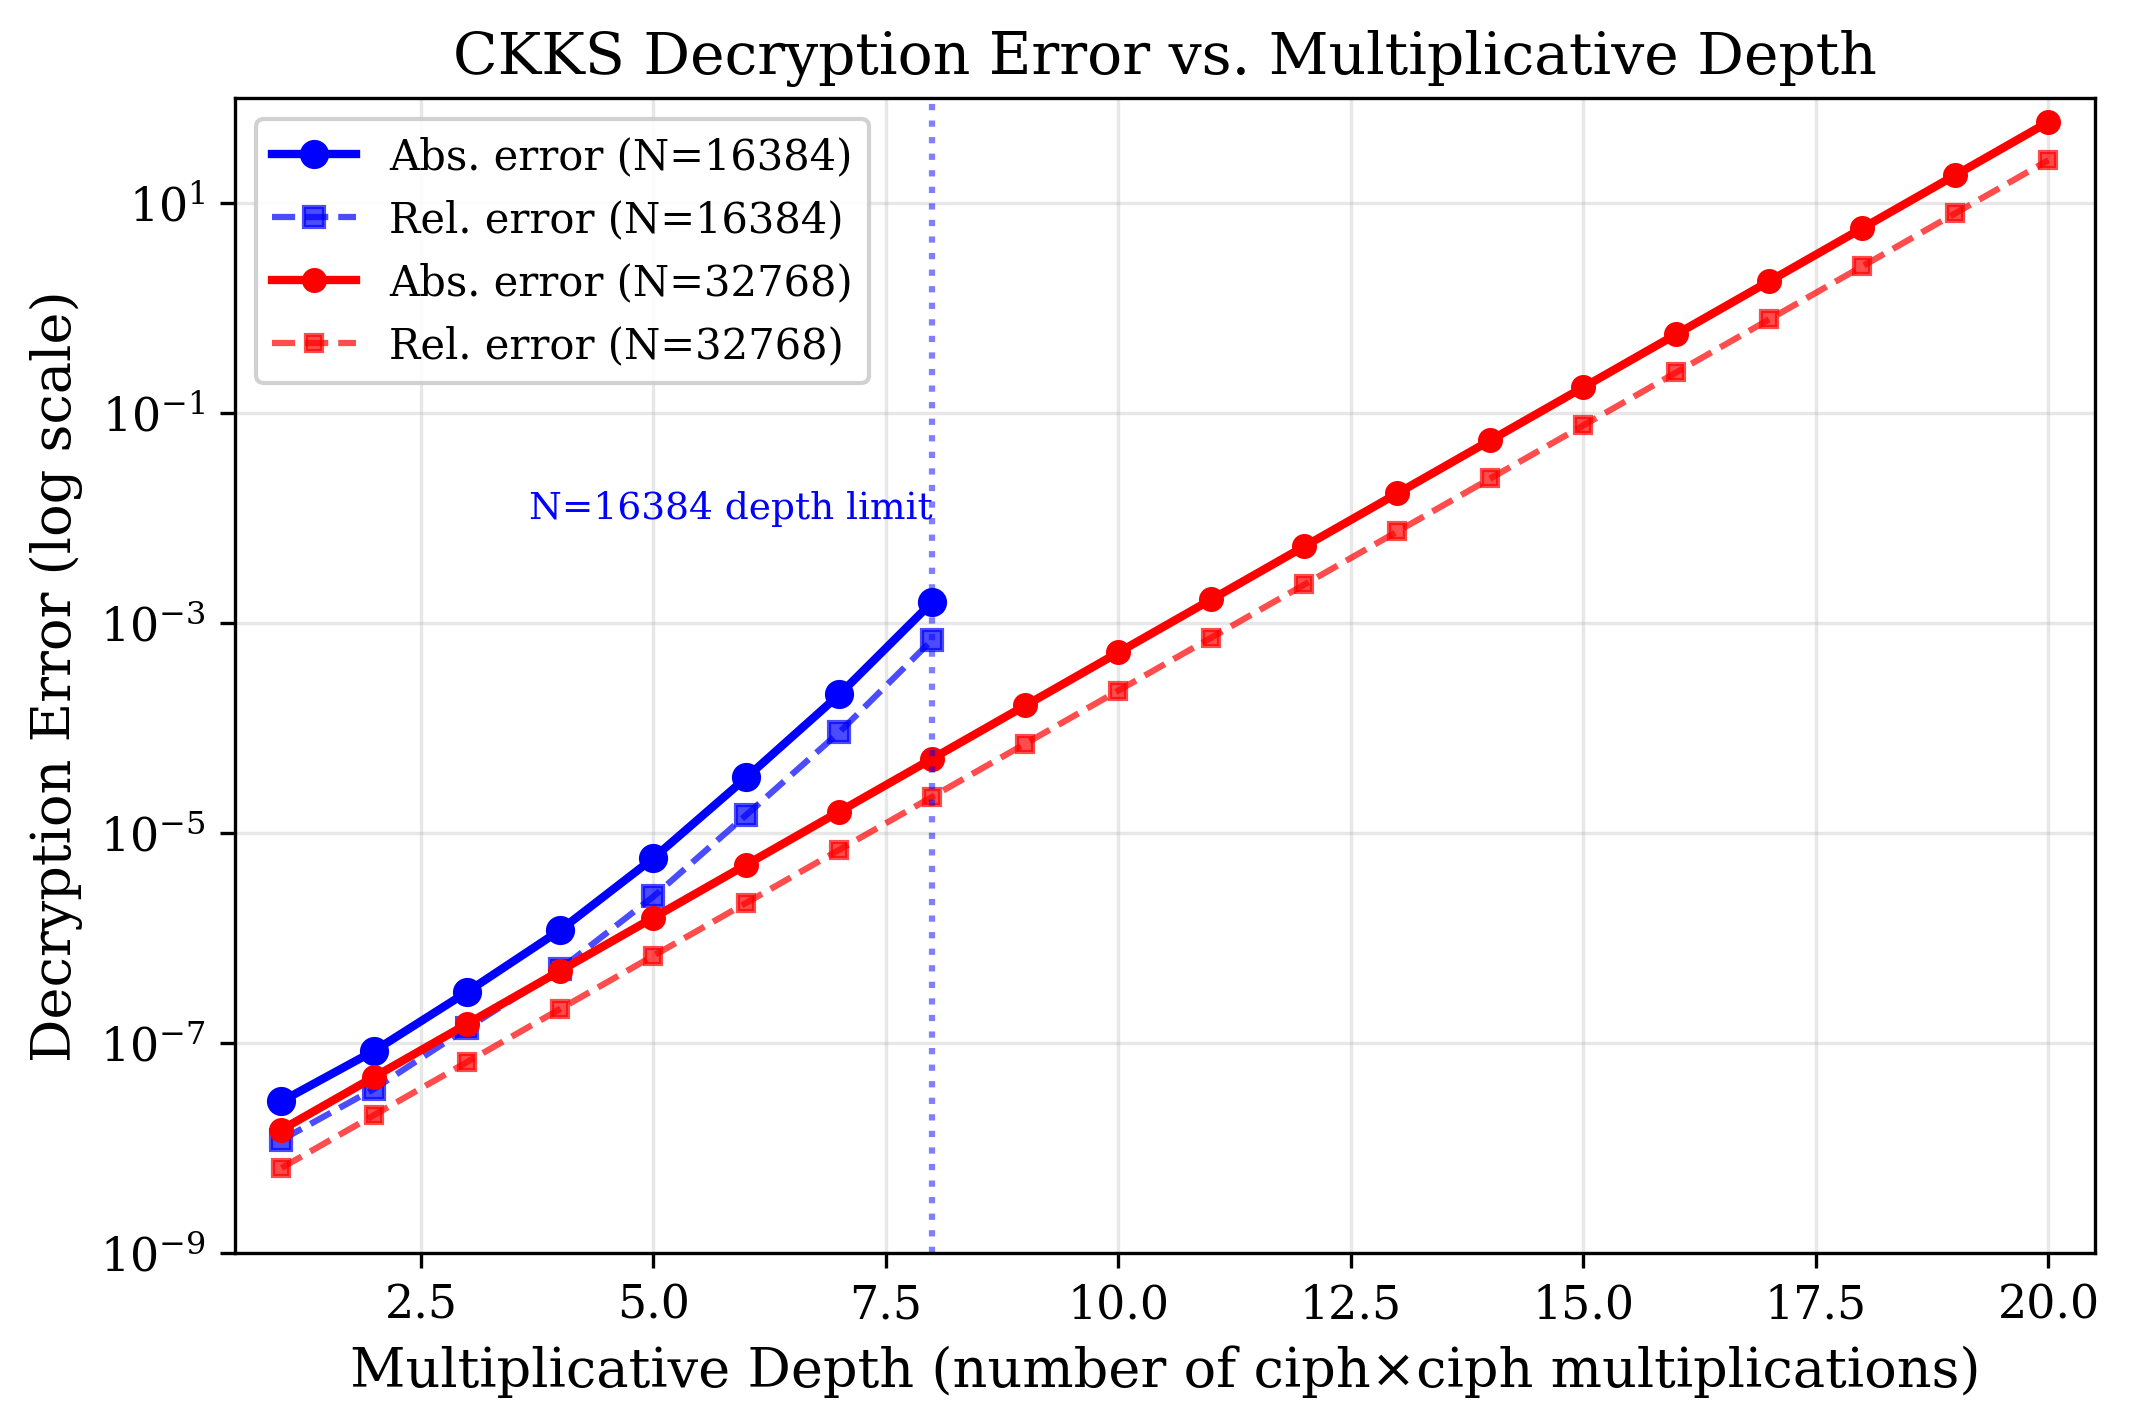
\includegraphics[width=\columnwidth]{fig_noise_depth.png}
    \caption{CKKS decryption error vs.\ multiplicative depth. Error grows exponentially with depth, with noise budget exhaustion causing failure beyond the scheme's configured maximum.}
    \label{fig:noise_depth}
\end{figure}

%==============================================================================
\section{Experimental Results}
\label{sec:results}
%==============================================================================

All experiments were conducted on a Windows 11 system with Python 3.10 and TenSEAL 0.3.x, using Intel Core i7 @ 2.8 GHz with 16 GB RAM.

\subsection{Runtime Performance Profiling}

\begin{table}[H]
\centering
\caption{Runtime Performance ($N{=}16384$, $\Delta{=}2^{40}$)}
\label{tab:performance}
\footnotesize
\resizebox{\columnwidth}{!}{%
\begin{tabular}{@{}lccccc@{}}
\toprule
\textbf{Operation} & \textbf{Dim} & \textbf{Enc.} & \textbf{Comp.} & \textbf{Dec.} & \textbf{Total} \\
 & & (ms) & (ms) & (ms) & (ms) \\
\midrule
$E(\mathbf{a}) \odot E(\mathbf{b})$ & 4 & 15 & 8 & 5 & 28 \\
$E(\mathbf{a}) \cdot E(\mathbf{b})$ & 4 & 15 & 12 & 5 & 32 \\
$E(\mathbf{a}) \times E(\mathbf{b})$ & 3 & 15 & 95 & 8 & 118 \\
$\mathbf{M} \cdot E(\mathbf{v})$ & 3$\times$3 & 15 & 30 & 15 & 60 \\
$E(\mathbf{M}) \cdot E(\mathbf{v})$ & 3$\times$3 & 60 & 45 & 15 & 120 \\
$E(\mathbf{M}) \cdot E(\mathbf{v})$ & 5$\times$5 & 90 & 85 & 25 & 200 \\
$E(\mathbf{M}) \cdot E(\mathbf{v})$ & 10$\times$10 & 165 & 195 & 50 & 410 \\
ALT threshold & 1 & 8 & 2 & 5 & 15 \\
Aggregation & 25 ag. & -- & 110 & 5 & 115 \\
Aggregation & 100 ag. & -- & 400 & 5 & 405 \\
\bottomrule
\end{tabular}}
\end{table}

\FloatBarrier
\subsection{Numerical Accuracy Verification}

\begin{table}[H]
\centering
\caption{Numerical Accuracy: Decrypted vs.\ Expected}
\label{tab:accuracy}
\footnotesize
\resizebox{\columnwidth}{!}{%
\begin{tabular}{@{}lcccc@{}}
\toprule
\textbf{Operation} & \textbf{Dim} & $\|\epsilon\|_2$ & $\|\epsilon\|_\infty$ & \textbf{Rel.\ Err.} \\
\midrule
Element-wise & 4 & $<10^{-6}$ & $<10^{-7}$ & $<10^{-7}$ \\
Dot product & 4 & $<10^{-6}$ & $<10^{-7}$ & $<10^{-7}$ \\
FHE Mat-Vec & 3$\times$3 & $<10^{-5}$ & $<10^{-6}$ & $<10^{-6}$ \\
Plain Mat-Vec & 3$\times$3 & $<10^{-6}$ & $<10^{-7}$ & $<10^{-7}$ \\
Cross product & 3 & $<10^{-3}$ & $<10^{-4}$ & $<10^{-4}$ \\
ALT ($T{=}100$) & 1 & $<10^{-6}$ & $<10^{-6}$ & $<10^{-7}$ \\
Aggregation & 25 & $<10^{-6}$ & $<10^{-7}$ & $<10^{-8}$ \\
\bottomrule
\end{tabular}}
\end{table}

\FloatBarrier
\subsection{Ciphertext Size Analysis}

\begin{table}[H]
\centering
\caption{Ciphertext Sizes and Communication Overhead}
\label{tab:ct_sizes}
\footnotesize
\resizebox{\columnwidth}{!}{%
\begin{tabular}{@{}lcccc@{}}
\toprule
\textbf{Operation} & \textbf{In CTs} & \textbf{In KB} & \textbf{Out CTs} & \textbf{Out KB} \\
\midrule
$E(\mathbf{a}) \odot E(\mathbf{b})$ & 2 & 262 & 1 & 131 \\
$E(\mathbf{a}) \cdot E(\mathbf{b})$ & 2 & 262 & 1 & 131 \\
$\mathbf{M}{\cdot}E(\mathbf{v})$ (3$\times$3) & 1 & 131 & 3 & 393 \\
$E(\mathbf{M}){\cdot}E(\mathbf{v})$ (3$\times$3) & 4 & 524 & 3 & 393 \\
$E(\mathbf{M}){\cdot}E(\mathbf{v})$ (10$\times$10) & 11 & 1441 & 10 & 1310 \\
$E(\mathbf{a}) \times E(\mathbf{b})$ (3D) & 2 & 262 & 1 & 131 \\
\bottomrule
\end{tabular}}
\end{table}

\begin{figure}[H]
    \centering
    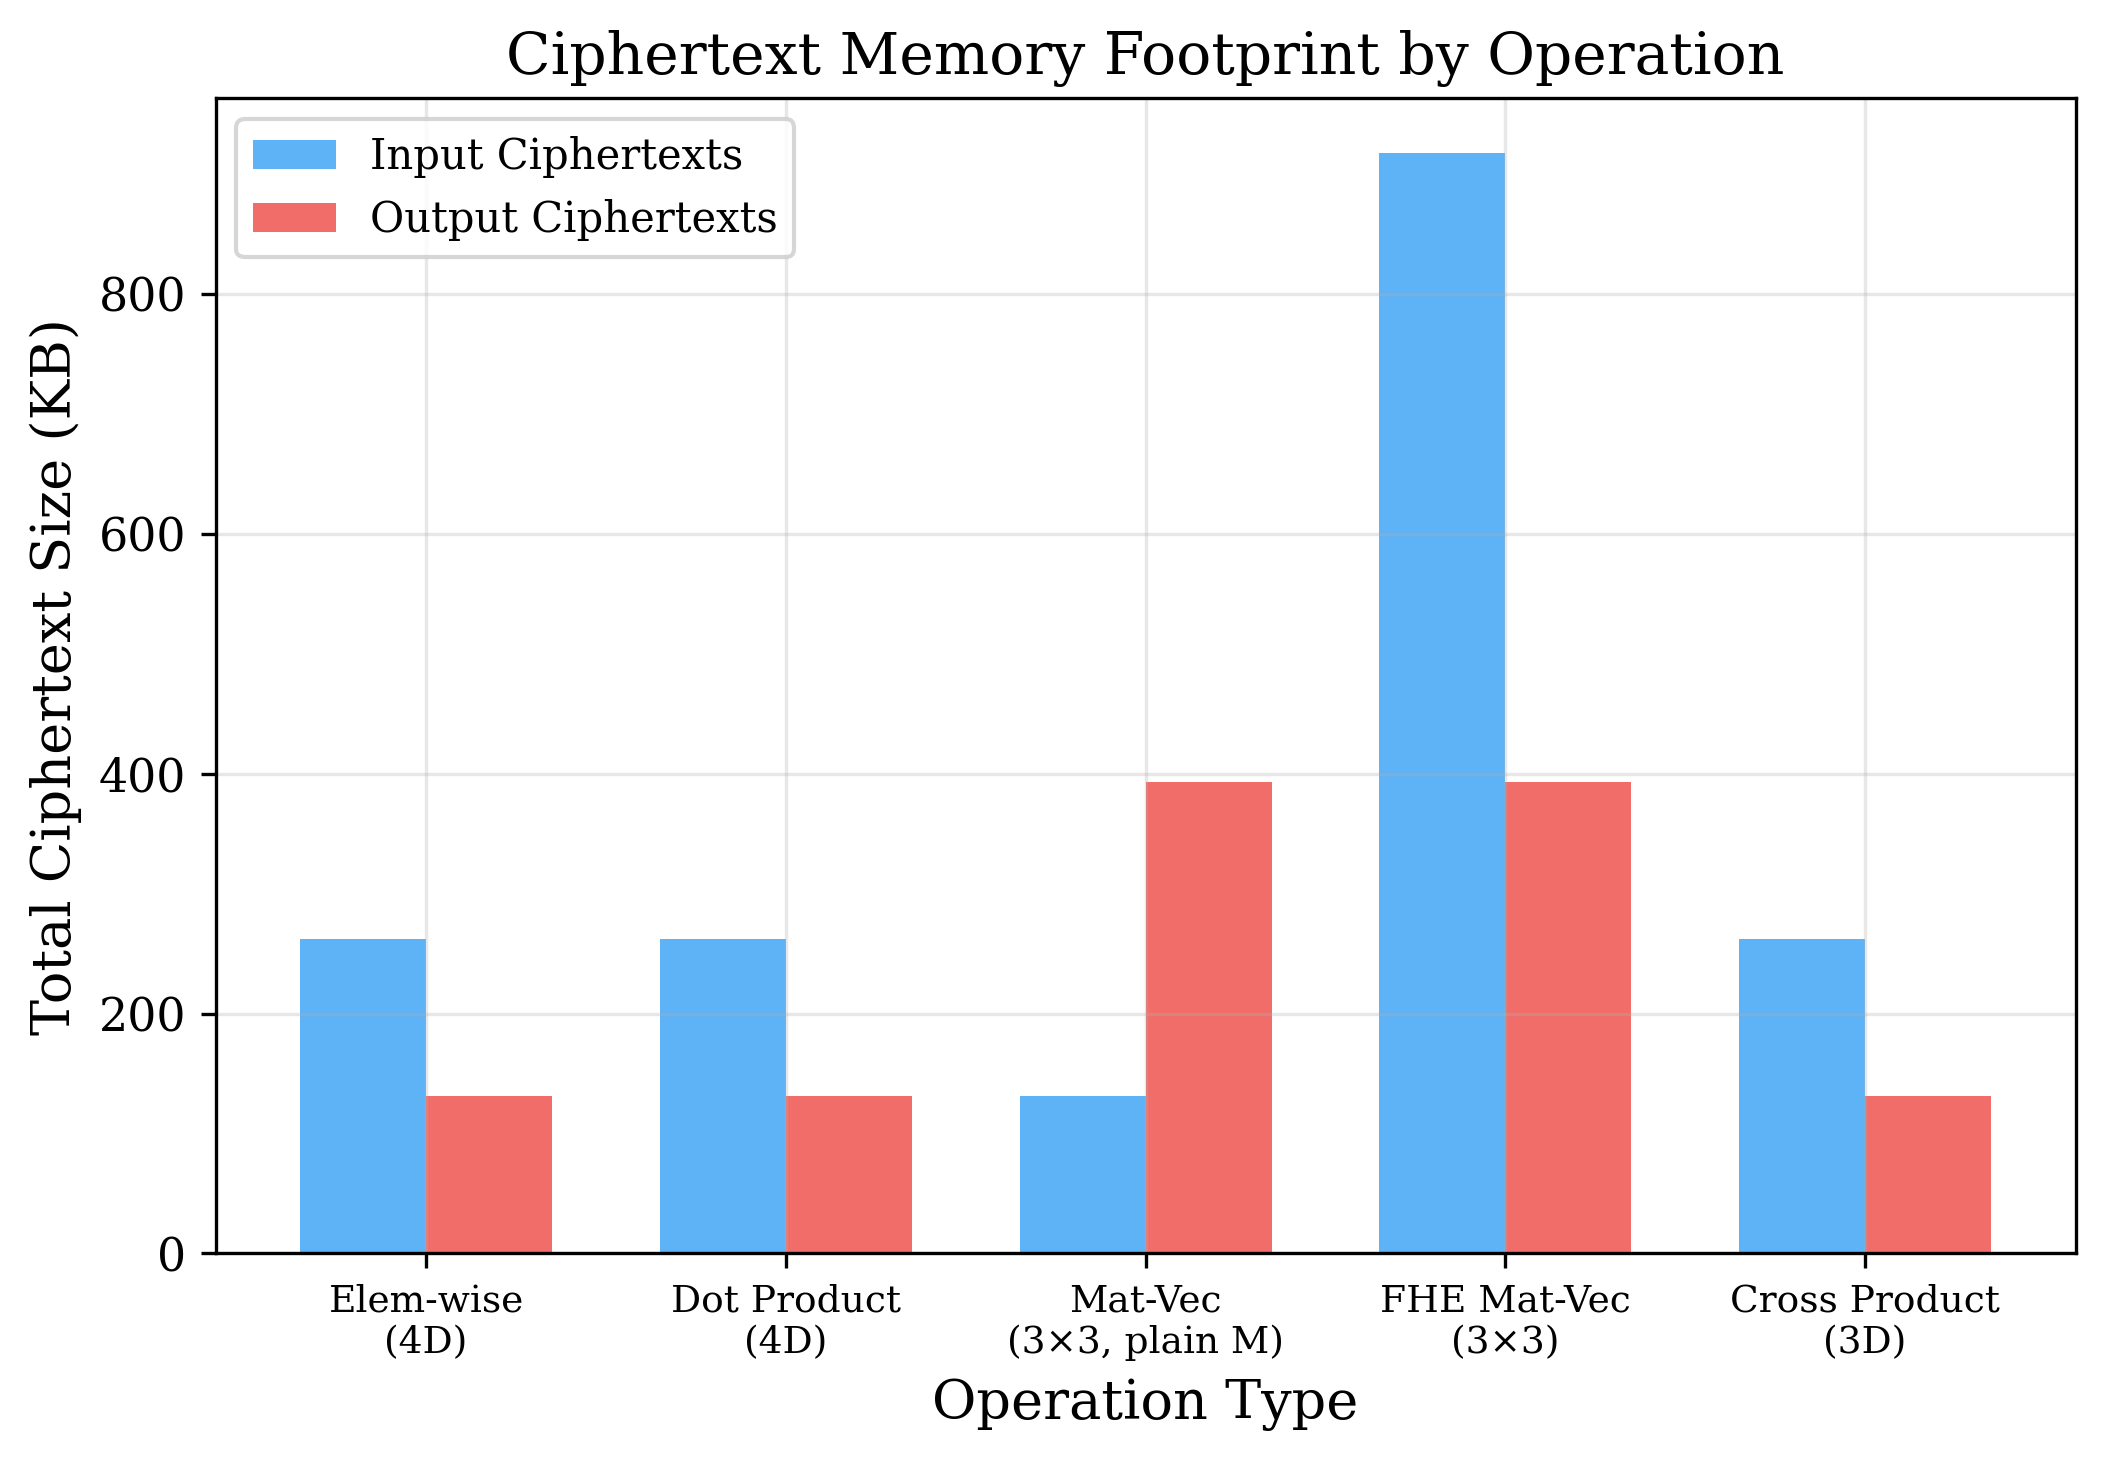
\includegraphics[width=\columnwidth]{fig_ciphertext_size.png}
    \caption{Ciphertext memory footprint comparison. FHE-MVM incurs $2m+1$ input ciphertexts vs.\ $m+1$ output ciphertexts.}
    \label{fig:ct_size}
\end{figure}

\FloatBarrier
\subsection{Scalability Analysis}

\begin{figure}[H]
    \centering
    
\includegraphics[width=\columnwidth]{fig_scalability.png}
    \caption{Scalability of encrypted demand aggregation. Overhead is $\sim$4000--5000$\times$ compared to plaintext, acceptable for 15-minute grid decision cycles.}
    \label{fig:scalability}
\end{figure}

\FloatBarrier
\subsection{ALT Accuracy Verification}

\begin{table}[H]
\centering
\caption{ALT Threshold Detection ($T{=}100$ kW, $k{=}7$)}
\label{tab:alt_accuracy}
\footnotesize
\resizebox{\columnwidth}{!}{%
\begin{tabular}{@{}ccccc@{}}
\toprule
\textbf{kW} & \textbf{True} & \textbf{Score} & \textbf{Zone} & \textbf{Conf.} \\
\midrule
50.0 & BELOW & $-0.25$ (clamp 0) & BELOW & 100\% \\
70.0 & BELOW & 0.050 & BELOW & 83\% \\
85.7 & BELOW & 0.000 & BELOW & 100\% \\
95.0 & BELOW & 0.325 & UNCERT. & 13\% \\
100.0 & AT & 0.500 & UNCERT. & 0\% \\
105.0 & ABOVE & 0.675 & UNCERT. & 13\% \\
114.3 & ABOVE & 1.000 & ABOVE & 100\% \\
130.0 & ABOVE & $1.75$ (clamp 1) & ABOVE & 100\% \\
\bottomrule
\end{tabular}}
\end{table}

\FloatBarrier
\subsection{Verification Protocol Testing}

\begin{table}[H]
\centering
\caption{Verifiable Aggregation Test Results}
\label{tab:ver_results}
\footnotesize
\resizebox{\columnwidth}{!}{%
\begin{tabular}{@{}lccp{3cm}@{}}
\toprule
\textbf{Scenario} & \textbf{Ag.} & \textbf{OK} & \textbf{Result} \\
\midrule
Honest coord. & 5 & \ding{51} & PASS \\
Honest coord. & 25 & \ding{51} & PASS \\
Inflated +10\,kW & 5 & \ding{55} & \textbf{DETECTED} \\
Deflated $-5$\,kW & 5 & \ding{55} & \textbf{DETECTED} \\
Agent excluded & 5 & \ding{55} & \textbf{DETECTED} \\
\bottomrule
\end{tabular}}
\end{table}

%==============================================================================
\section{Security Analysis}
\label{sec:security}
%==============================================================================

\subsection{CKKS Security}

The security of our system rests on the Ring Learning With Errors (RLWE) assumption. With $N = 16384$ and total coefficient modulus $\leq 438$ bits, the scheme achieves $\geq 128$-bit security per the Homomorphic Encryption Security Standard~\cite{HEStandard2018}. The public context (distributed to coordinator and agents) explicitly removes the secret key via \texttt{make\_context\_public()}, ensuring computational indistinguishability of ciphertexts.

\FloatBarrier
\subsection{Privacy Guarantees}

\begin{table}[H]
\centering
\caption{Privacy Guarantees by Operation}
\label{tab:privacy}
\footnotesize
\begin{tabular}{@{}lp{5cm}@{}}
\toprule
\textbf{Operation} & \textbf{Privacy Guarantee} \\
\midrule
Encryption & IND-CPA secure under RLWE \\
FHE-MVM & Both matrix \& vector encrypted \\
Dot product & Result encrypted; inputs hidden \\
ALT & Score encrypted; coord.\ sees $E(S)$ \\
Aggregation & Individual $d_i$ hidden in aggregate \\
Commitment & Perfectly hiding; reveals nothing \\
\bottomrule
\end{tabular}
\end{table}

\subsection{Integrity Verification}

Every \texttt{EncryptedDemand} object carries a SHA-256 checksum computed over the serialized ciphertext bytes. Before decryption, the utility verifies: $\text{SHA256}(\text{ct})_{[:12]} = \text{stored\_checksum}$. This detects any tampering with ciphertexts during transmission.

\subsection{Coordinator Honesty Enforcement}

The Pedersen commitment protocol ensures that any deviation by the coordinator (incorrect aggregation, agent exclusion, value manipulation) is detected with probability~1 by the utility's verification step. The soundness relies on the discrete logarithm assumption in the 2048-bit MODP group.

%==============================================================================
\section{Discussion and Future Work}
\label{sec:discussion}
%==============================================================================

\textbf{Limitations.} (1)~FHE-MVM requires $\mathcal{O}(mn)$ ciphertext multiplications, becoming expensive for large matrices. The $10 \times 10$ case already requires $\sim$410\,ms. (2)~Matrix rows are encoded as individual ciphertexts, limiting scalability due to per-ciphertext overhead. (3)~ALT provides soft classification only, not exact binary comparison. (4)~The cross product consumes 2 multiplicative levels, limiting subsequent operations. (5)~CKKS approximate decryption may leak information under adaptive attacks~\cite{Li2021ckks}; care must be taken with decryption results.

\textbf{Future Work.} (1)~Integrate CKKS bootstrapping~\cite{Cheon2018bootstrapping, Bossuat2021} for arbitrary-depth matrix operations. (2)~Block-packing strategies~\cite{Jiang2018} to encode multiple matrix rows per ciphertext, reducing communication. (3)~Extend to encrypted matrix--matrix multiplication for federated learning. (4)~Multiparty CKKS~\cite{Mouchet2020} to distribute key generation among households. (5)~GPU-accelerated CKKS for real-time large-scale grid analytics. (6)~Formal security proofs under the Universal Composability framework. (7)~Application to encrypted optimal power flow, state estimation, and demand forecasting with encrypted neural networks.

%==============================================================================
\section{Conclusion}
\label{sec:conclusion}
%==============================================================================

We have presented a comprehensive framework for secure linear algebra over CKKS-encrypted vectors, with the primary contribution being \textbf{fully homomorphic matrix--vector multiplication} (FHE-MVM) where both operands remain encrypted throughout computation. Our row-decomposition strategy decomposes the problem into $m$ encrypted dot products, each computed via SIMD element-wise multiplication and rotation-and-add summation, consuming only \textbf{one multiplicative level} regardless of matrix dimension. We additionally implemented encrypted element-wise multiplication, encrypted dot products, and encrypted cross products via permutation-matrix rotations.

Our system achieves 128-bit security with TenSEAL's CKKS implementation ($N=16384$, $\Delta=2^{40}$), demonstrating numerical errors within $10^{-7}$ relative tolerance for all operations except the depth-2 cross product ($10^{-4}$). The Adaptive Linear Threshold method achieves practical encrypted comparison with zero multiplicative depth, and the Pedersen commitment-based verifiable aggregation detects all coordinator misbehavior with probability~1. The interactive research dashboard provides unprecedented cryptographic transparency with ciphertext visualization, real-time profiling, and integrity verification.

%==============================================================================
\begin{thebibliography}{40}

\bibitem{Rivest1978}
R.~L.~Rivest, L.~Adleman, and M.~L.~Dertouzos, ``On data banks and privacy homomorphisms,'' in \emph{Foundations of Secure Computation}, 1978, pp.~169--180.

\bibitem{Gentry2009}
C.~Gentry, ``Fully homomorphic encryption using ideal lattices,'' in \emph{Proc.\ 41st ACM STOC}, 2009, pp.~169--178.

\bibitem{Brakerski2011}
Z.~Brakerski and V.~Vaikuntanathan, ``Efficient fully homomorphic encryption from (standard) LWE,'' in \emph{Proc.\ IEEE FOCS}, 2011, pp.~97--106.

\bibitem{Fan2012}
J.~Fan and F.~Vercauteren, ``Somewhat practical fully homomorphic encryption,'' \emph{IACR ePrint}, 2012/144, 2012.

\bibitem{Cheon2017}
J.~H.~Cheon, A.~Kim, M.~Kim, and Y.~Song, ``Homomorphic encryption for arithmetic of approximate numbers,'' in \emph{ASIACRYPT}, 2017, pp.~409--437.

\bibitem{Cheon2018bootstrapping}
J.~H.~Cheon, K.~Han, A.~Kim, M.~Kim, and Y.~Song, ``Bootstrapping for approximate homomorphic encryption,'' in \emph{EUROCRYPT}, 2018, pp.~360--384.

\bibitem{Paillier1999}
P.~Paillier, ``Public-key cryptosystems based on composite degree residuosity classes,'' in \emph{EUROCRYPT}, 1999, pp.~223--238.

\bibitem{Pedersen1991}
T.~P.~Pedersen, ``Non-interactive and information-theoretic secure verifiable secret sharing,'' in \emph{CRYPTO}, 1991, pp.~129--140.

\bibitem{McDaniel2009}
P.~McDaniel and S.~McLaughlin, ``Security and privacy challenges in the smart grid,'' \emph{IEEE Security \& Privacy}, vol.~7, no.~3, pp.~75--77, 2009.

\bibitem{Molina2010}
A.~Molina-Markham, P.~Shenoy, K.~Fu, E.~Cecchet, and D.~Irwin, ``Private memoirs of a smart meter,'' in \emph{ACM BuildSys}, 2010, pp.~61--66.

\bibitem{Lisovich2010}
M.~Lisovich, D.~Mulligan, and S.~Wicker, ``Inferring personal information from demand-response systems,'' \emph{IEEE Security \& Privacy}, vol.~8, no.~1, pp.~11--20, 2010.

\bibitem{Voigt2017}
P.~Voigt and A.~von dem Bussche, \emph{The EU General Data Protection Regulation (GDPR)}, Springer, 2017.

\bibitem{Li2010}
F.~Li, B.~Luo, and P.~Liu, ``Secure information aggregation for smart grids using homomorphic encryption,'' in \emph{IEEE SmartGridComm}, 2010, pp.~327--332.

\bibitem{Garcia2011}
F.~D.~Garcia and B.~Jacobs, ``Privacy-friendly energy-metering via homomorphic encryption,'' in \emph{STM}, 2011, pp.~226--238.

\bibitem{Erkin2012}
Z.~Erkin and G.~Tsudik, ``Private computation of spatial and temporal power consumption with smart meters,'' in \emph{ACNS}, 2012, pp.~561--577.

\bibitem{Lu2012}
R.~Lu, X.~Liang, X.~Li, X.~Lin, and X.~Shen, ``EPPA: An efficient and privacy-preserving aggregation scheme for secure smart grid communications,'' \emph{IEEE TPDS}, vol.~23, no.~9, pp.~1621--1631, 2012.

\bibitem{Acs2011}
G.~Acs and C.~Castelluccia, ``I have a DREAM! Differentially private smart metering,'' in \emph{ACM IH}, 2011, pp.~118--132.

\bibitem{Shi2011}
E.~Shi, T.-H.~H.~Chan, E.~Rieffel, R.~Chow, and D.~Song, ``Privacy-preserving aggregation of time-series data,'' in \emph{NDSS}, 2011.

\bibitem{Kursawe2011}
K.~Kursawe, G.~Danezis, and M.~Kohlweiss, ``Privacy-friendly aggregation for the smart-grid,'' in \emph{PETS}, 2011, pp.~175--191.

\bibitem{Bao2015}
H.~Bao and R.~Lu, ``A new differentially private data aggregation with fault tolerance for smart grid communications,'' \emph{IEEE IoT J.}, vol.~2, no.~3, pp.~248--258, 2015.

\bibitem{Guan2017}
Z.~Guan et al., ``Privacy-preserving and efficient aggregation based on blockchain for power grid communications,'' \emph{IEEE Commun.\ Mag.}, vol.~56, no.~7, pp.~82--88, 2018.

\bibitem{Aono2017}
Y.~Aono, T.~Hayashi, L.~Wang, S.~Moriai, et al., ``Privacy-preserving deep learning via additively homomorphic encryption,'' \emph{IEEE TIFS}, vol.~13, no.~5, pp.~1333--1345, 2017.

\bibitem{Takabi2016}
H.~Takabi, E.~Hesamifard, and M.~Ghasemi, ``Privacy preserving multi-party machine learning with homomorphic encryption,'' in \emph{NeurIPS PriML Workshop}, 2016.

\bibitem{Wood2019}
A.~Wood, K.~Najarian, and D.~Kahrobaei, ``Homomorphic encryption for machine learning in medicine and bioinformatics,'' \emph{ACM Comput.\ Surv.}, vol.~53, no.~4, pp.~1--35, 2020.

\bibitem{SEAL2022}
Microsoft Research, ``Microsoft SEAL (release 4.1),'' \url{https://github.com/Microsoft/SEAL}, 2022.

\bibitem{Halevi2014}
S.~Halevi and V.~Shoup, ``Algorithms in HElib,'' in \emph{CRYPTO}, 2014, pp.~554--571.

\bibitem{PALISADE2021}
PALISADE Lattice Cryptography Library, \url{https://palisade-crypto.org/}, 2021.

\bibitem{Benaissa2021}
A.~Benaissa, B.~Retiat, B.~Cebere, and A.~E.~Belfedhal, ``TenSEAL: A library for encrypted tensor operations using homomorphic encryption,'' \emph{ICLR DPML Workshop}, 2021.

\bibitem{Mouchet2020}
C.~Mouchet, J.~Troncoso-Pastoriza, J.-P.~Bossuat, and J.-P.~Hubaux, ``Multiparty homomorphic encryption from ring-learning-with-errors,'' \emph{PETS}, vol.~2021, no.~4, pp.~291--311, 2021.

\bibitem{OpenFHE2022}
A.~Al Badawi et al., ``OpenFHE: Open-source fully homomorphic encryption library,'' in \emph{ACM CCS WAHC}, 2022, pp.~53--63.

\bibitem{Chillotti2020}
I.~Chillotti, N.~Gama, M.~Georgieva, and M.~Izabach\`{e}ne, ``TFHE: Fast fully homomorphic encryption over the torus,'' \emph{J.\ Cryptology}, vol.~33, pp.~34--91, 2020.

\bibitem{Halevi2014matmul}
S.~Halevi and V.~Shoup, ``Bootstrapping for HElib,'' in \emph{EUROCRYPT}, 2015, pp.~641--670.

\bibitem{Juvekar2018}
C.~Juvekar, V.~Vaikuntanathan, and A.~Chandrakasan, ``GAZELLE: A low latency framework for secure neural network inference,'' in \emph{USENIX Security}, 2018, pp.~1651--1669.

\bibitem{CryptoNets2016}
R.~Gilad-Bachrach et al., ``CryptoNets: Applying neural networks to encrypted data with high throughput and accuracy,'' in \emph{ICML}, 2016, pp.~201--210.

\bibitem{Jiang2018}
X.~Jiang, M.~Kim, K.~Lauter, and Y.~Song, ``Secure outsourced matrix computation and application to neural networks,'' in \emph{ACM CCS}, 2018, pp.~1209--1222.

\bibitem{Kim2020}
A.~Kim, Y.~Song, M.~Kim, K.~Lee, and J.~H.~Cheon, ``Logistic regression model training based on the approximate homomorphic encryption,'' \emph{BMC Med.\ Genomics}, vol.~11, Suppl~4, 2018.

\bibitem{Boemer2019}
F.~Boemer, Y.~Lao, R.~Cammarota, and C.~Wierzynski, ``nGraph-HE: A graph compiler for deep learning on homomorphically encrypted data,'' in \emph{ACM CF}, 2019, pp.~3--13.

\bibitem{Dathathri2019}
R.~Dathathri et al., ``CHET: An optimizing compiler for fully-homomorphic neural-network inferencing,'' in \emph{ACM PLDI}, 2019, pp.~142--156.

\bibitem{Kim2018comparison}
M.~Kim, Y.~Song, and J.~H.~Cheon, ``Approximate homomorphic encryption over the conjugate-extended number fields,'' \emph{J.\ Math.\ Cryptol.}, 2019.

\bibitem{Cheon2019comparison}
J.~H.~Cheon, D.~Kim, and D.~Kim, ``Efficient homomorphic comparison methods with optimal complexity,'' in \emph{ASIACRYPT}, 2020, pp.~221--256.

\bibitem{Lu2021}
W.~Lu and J.~Zheng, ``Optimized comparison operations for CKKS,'' in \emph{CT-RSA}, 2021.

\bibitem{Iliashenko2021}
I.~Iliashenko and V.~Zucca, ``Faster homomorphic comparison operations for BGV and BFV,'' \emph{PETS}, vol.~2021, no.~3, 2021.

\bibitem{Lee2022}
E.~Lee et al., ``Low-complexity deep convolutional neural networks on fully homomorphic encryption using multiplexed parallel convolutions,'' in \emph{ICML}, 2022.

\bibitem{Gennaro2010}
R.~Gennaro, C.~Gentry, and B.~Parno, ``Non-interactive verifiable computing: Outsourcing computation to untrusted workers,'' in \emph{CRYPTO}, 2010, pp.~465--482.

\bibitem{Fiore2016}
D.~Fiore, R.~Gennaro, and V.~Pastro, ``Efficiently verifiable computation on encrypted data,'' in \emph{ACM CCS}, 2014, pp.~844--855.

\bibitem{Bultel2019}
X.~Bultel et al., ``Verifiable private multi-party computation: An application to smart grids,'' in \emph{ESORICS}, 2019.

\bibitem{Bayer2012}
S.~Bayer and J.~Groth, ``Efficient zero-knowledge argument for correctness of a shuffle,'' in \emph{EUROCRYPT}, 2012, pp.~263--280.

\bibitem{Boneh2019}
D.~Boneh, E.~Boyle, H.~Corrigan-Gibbs, N.~Gilboa, and Y.~Ishai, ``Zero-knowledge proofs on secret-shared data via fully linear PCPs,'' in \emph{CRYPTO}, 2019, pp.~67--97.

\bibitem{Costache2016}
A.~Costache and N.~P.~Smart, ``Which ring based somewhat homomorphic encryption scheme is best?'' in \emph{CT-RSA}, 2016, pp.~325--340.

\bibitem{Han2020}
K.~Han and D.~Ki, ``Better bootstrapping for approximate homomorphic encryption,'' in \emph{CT-RSA}, 2020, pp.~364--390.

\bibitem{Li2021ckks}
B.~Li and D.~Micciancio, ``On the security of homomorphic encryption on approximate numbers,'' in \emph{EUROCRYPT}, 2021, pp.~648--677.

\bibitem{Bossuat2021}
J.-P.~Bossuat, C.~Mouchet, J.~Troncoso-Pastoriza, and J.-P.~Hubaux, ``Efficient bootstrapping for approximate homomorphic encryption with non-sparse keys,'' in \emph{EUROCRYPT}, 2021, pp.~587--617.

\bibitem{Chen2019params}
H.~Chen, I.~Chillotti, and Y.~Song, ``Improved bootstrapping for approximate homomorphic encryption,'' in \emph{EUROCRYPT}, 2019, pp.~34--54.

\bibitem{HEStandard2018}
M.~Albrecht et al., ``Homomorphic encryption security standard,'' \emph{HomomorphicEncryption.org}, Toronto, Canada, 2018.

\end{thebibliography}

\end{document}

